% Compile with XeLaTeX:
% xelatex final_report_a4_en.tex
\documentclass[a4paper,11pt]{article}
\usepackage[a4paper,margin=2.2cm]{geometry}
\usepackage{amsmath,booktabs,graphicx,xcolor,hyperref,float}
\hypersetup{colorlinks=true,linkcolor=blue,urlcolor=blue}
\title{Perspective-Correct Texture Mapping and Budgeted Collaborative Filtering}
\author{Computer Graphics Course Project\\Team members: to be added}
\date{November 24, 2026}
\begin{document}
\maketitle

\begin{abstract}
This project implements a small CPU triangle rasterizer and compares screen-space affine UV interpolation with perspective-correct UV interpolation. A planar quad is rotated around the vertical axis at $0^\circ$, $15^\circ$, $30^\circ$, $45^\circ$, $60^\circ$, and $70^\circ$ while a generated checkerboard texture is rendered. The error grows as the plane becomes more oblique: at $70^\circ$, the mean UV error is 29.54 texture pixels and the 95th-percentile error is 49.80 texture pixels.

A second experiment keeps the perspective-correct UV fixed and compares three Catmull--Rom reconstructions on the same pixels: the exact 16-tap filter, a two-tap stochastic estimator, and Mask Sampling with the C+ fallback from Collaborative Texture Filtering (HPG 2025). Each aligned $8\times4$ tile may use at most one texel evaluation per active pixel. At a $32\times32$ texture and $0^\circ$, every full tile is exact, the collaborative filter uses 0.61 evaluations per pixel, and its mean PSNR against the 16-tap filter is 58.22~dB. The two-tap estimator uses 2 evaluations and reaches 14.32~dB. Once magnification falls below one, exact tiles disappear and the advantage shrinks to about 1.5~dB.
\end{abstract}

\section{Introduction}
A rasterizer converts projected triangles into pixels and computes color, depth, and texture coordinates for each covered pixel. Under perspective projection, screen-space distance is not linear with distance on the original 3D surface. Directly interpolating UV coordinates in screen space therefore produces texture stretching and compression.

This project builds a small CPU triangle rasterizer and asks two questions. First, how does the error of affine UV interpolation change as a textured plane rotates into perspective? The camera, geometry, texture, coverage test, and depth buffer remain fixed; only the UV interpolation rule changes. Second, once the UV is perspective-correct, can a one-evaluation-per-pixel collaborative filter reproduce a 16-tap Catmull--Rom reconstruction? The rasterizer answers the first question by rendering one textured plane under both UV rules. It answers the second by applying Mask Sampling and the C+ fallback, together with a two-tap baseline, to that perspective-correct UV.

\section{Related Work}
Lectures 03--06 cover rasterization, spatial transformations, perspective projection, and texture mapping. These topics form the rendering pipeline implemented here. The OpenGL GLSL specification describes \texttt{smooth} interpolation as perspective-correct and \texttt{noperspective} interpolation as linear in screen space. The Vulkan specification gives the corresponding reciprocal-$w$ rule for triangle data interpolation.

The reconstruction experiment follows Collaborative Texture Filtering~\cite{ctf}. That method lets the lanes of an $8\times4$ GPU wave share texel evaluations so that a discrete filter can be exact when one evaluation per lane is enough. When the merged footprint does not fit, their C+ fallback spends the remaining lanes on missing taps and completes the filter with a biased fill-in. The comparison baseline is a two-tap stochastic estimator for a signed kernel, the Catmull--Rom setting discussed in that paper and descending from stochastic texture filtering~\cite{stf}. The implementation here is a CPU model of the same tile decision. It uses ordinary array lookups rather than wave intrinsics, and it does not include a neural decoder or a denoiser.

\section{Methods}
The scene contains one planar quad of size $2.7\times1.9$ units, split into two triangles. The model rotates around the vertical axis and uses a $52^\circ$ perspective projection. The output is $512\times512$ pixels. The texture is a generated $256\times256$ checkerboard with $12\times12$ cells and nearest-neighbor sampling.

Let $\lambda_0,\lambda_1,\lambda_2$ be screen-space barycentric coordinates, $uv_i$ the vertex texture coordinates, and $w_i$ the clip-space homogeneous coordinate. Affine interpolation is
\begin{equation}
uv_{\mathrm{affine}}=\lambda_0uv_0+\lambda_1uv_1+\lambda_2uv_2.
\end{equation}
Perspective-correct interpolation is
\begin{equation}
uv_{\mathrm{perspective}}=
\frac{\sum_i\lambda_i uv_i/w_i}{\sum_i\lambda_i/w_i}.
\end{equation}

The rasterization pipeline transforms vertices to clip and screen space, tests pixel-center coverage with edge functions and barycentric coordinates, interpolates depth for a software Z-buffer, evaluates one of the two UV formulas, and samples the checkerboard texture. Table~\ref{tab:settings} lists the settings held fixed while the plane rotates.

\begin{table}[H]
\centering
\caption{Experiment settings}
\label{tab:settings}
\begin{tabular}{ll}
\toprule
Item & Setting \\
\midrule
Output & $512\times512$ pixels \\
Geometry & One planar quad split into two triangles \\
Projection & $52^\circ$ field-of-view perspective projection \\
Texture & $256\times256$ pixels, $12\times12$ checkerboard \\
Angles & $0^\circ,15^\circ,30^\circ,45^\circ,60^\circ,70^\circ$ \\
Metrics & Mean UV error, P95 UV error, RGB MAE \\
\bottomrule
\end{tabular}
\end{table}

The UV comparison uses nearest-neighbor lookup, so its color error mixes coordinate error with texel boundaries. The second study removes that mixture. Every method reads the same perspective-correct UV buffer. The reference filter is separable Catmull--Rom with support $4\times4$:
\begin{equation}
C=\sum_{j=-1}^{2}\sum_{i=-1}^{2} k(t_x-i)\,k(t_y-j)\,T_{b_x+i,\,b_y+j},
\end{equation}
where $(b_x,b_y)$ is the texel-center origin $Nu-1/2$ and $(t_x,t_y)$ is the fractional offset. The kernel parameter is $a=-1/2$. An exact pixel therefore requests 16 texels.

Pixels are grouped into aligned $8\times4$ tiles, the wave shape used by the paper. Let $n$ be the number of covered pixels in a tile and $U$ the number of unique clamped taps in their footprints. If $U\le n$ and the unclamped footprint fits in a $16\times16$ window, Mask Sampling evaluates each unique texel once and applies the original weights. The reconstructed color then matches the 16-tap filter. Otherwise the tile uses the C+ fallback. Each active pixel draws one tap with probability proportional to the absolute Catmull--Rom weight, duplicate draws are replaced by missing taps in the same footprints, and known taps are combined by
\begin{equation}
\mathbf{c}=\sum_{i\in\mathcal{K}} w_i\mathbf{p}_i+\left(1-\sum_{i\in\mathcal{K}} w_i\right)\overline{\mathbf{p}}.
\end{equation}
Here $\mathcal{K}$ is the set of known texels and $\overline{\mathbf{p}}$ is their unweighted mean. A single known texel is returned directly, which is the paper's one-tap special case. This fallback is biased. The two-tap baseline is unbiased for the same cubic: it draws one positive-lobe sample and one negative-lobe sample and weights each by its lobe mass, for two evaluations per pixel.

The scene reuses the rasterizer at $0^\circ$, $45^\circ$, and $70^\circ$. Textures are $32^2$, $128^2$, and $512^2$ samples of three analytic signals: a low-frequency sum of sines, a higher-frequency sum of sines, and a 12-cell checker. Magnification is the median, over covered neighbor pairs, of the reciprocal of the larger screen-space texel derivative.

UV error is the Euclidean distance in texture-pixel coordinates, measured against the perspective-correct result on pixels covered by both modes. RGB MAE is averaged over the shared covered pixels and color channels on a 0--255 scale. Filter error is measured against the 16-tap color on every covered pixel. PSNR in Table~\ref{tab:sota} is the unweighted mean of the three per-texture PSNR values, and each of those is the mean of four random seeds. Analytic PSNR, against the continuous signal on pixels at least two texels from the texture border, is reported in the CSV and is a pointwise reference rather than an area integral.

\section{Results}
Figure~\ref{fig:comparison} shows the two outputs at $60^\circ$. Affine interpolation visibly stretches the checkerboard, while perspective-correct interpolation keeps the texture aligned with the projected surface.

\begin{figure}[H]
\centering
\begin{minipage}{0.47\textwidth}\centering
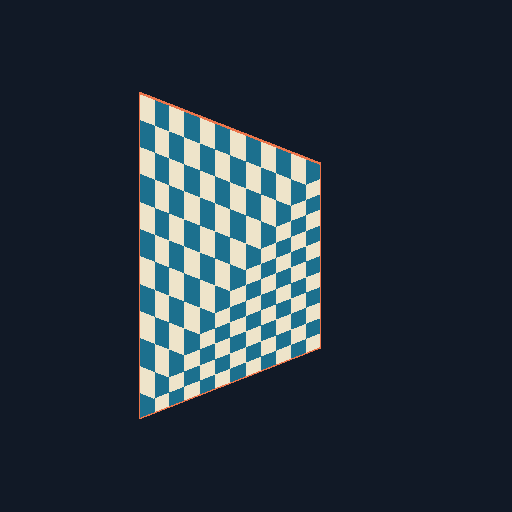
\includegraphics[width=\textwidth]{figures/angle_60_affine.png}\\Affine UV interpolation
\end{minipage}\hfill
\begin{minipage}{0.47\textwidth}\centering
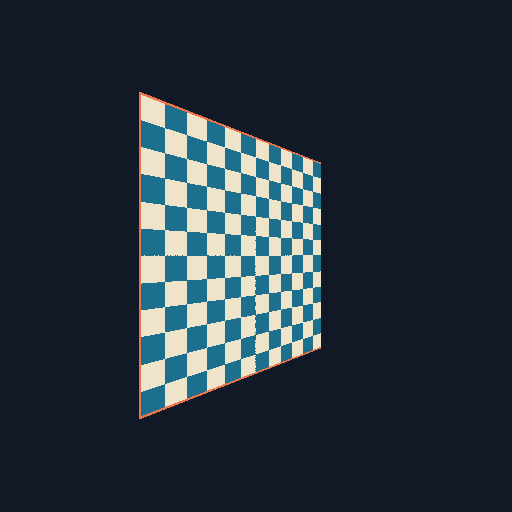
\includegraphics[width=\textwidth]{figures/angle_60_perspective.png}\\Perspective-correct UV interpolation
\end{minipage}
\caption{Texture comparison at a $60^\circ$ rotation angle}
\label{fig:comparison}
\end{figure}

\begin{table}[H]
\centering
\caption{Angle sweep results}
\label{tab:angles}
\begin{tabular}{rrrr}
\toprule
Angle & Mean UV (texels) & P95 UV (texels) & RGB MAE \\
\midrule
0 & 0.00 & 0.00 & 0.02 \\
15 & 8.14 & 13.47 & 46.43 \\
30 & 15.76 & 26.13 & 58.63 \\
45 & 22.18 & 37.14 & 57.02 \\
60 & 27.34 & 45.76 & 59.83 \\
70 & 29.54 & 49.80 & 60.68 \\
\bottomrule
\end{tabular}
\end{table}

Mean and P95 UV error increase with the rotation angle. At $70^\circ$, the mean UV error is 29.54 texture pixels and the P95 error is 49.80 texture pixels. RGB MAE is not perfectly monotonic because nearest-neighbor sampling changes abruptly at texel boundaries; UV error is the more direct measure of interpolation error.

\begin{table}[H]
\centering
\caption{Collaborative Catmull--Rom against the exact 16-tap filter. Full exact is the percentage of pixels in completely covered $8\times4$ tiles whose reconstruction matches that filter.}
\label{tab:sota}
\small
\begin{tabular}{rrrrrrr}
\toprule
Size & Angle & Mag. & Full exact & Evals/px & C+ (dB) & Two-tap (dB) \\
\midrule
32 & $0^\circ$ & 10.52 & 100\% & 0.61 & 58.22 & 14.32 \\
32 & $45^\circ$ & 8.23 & 100\% & 0.64 & 55.09 & 14.33 \\
32 & $70^\circ$ & 6.63 & 90.9\% & 0.74 & 57.31 & 14.35 \\
128 & $0^\circ$ & 2.63 & 19.9\% & 0.98 & 57.28 & 23.31 \\
128 & $45^\circ$ & 2.06 & 9.6\% & 0.99 & 48.75 & 23.30 \\
128 & $70^\circ$ & 1.66 & 0.0\% & 1.00 & 35.90 & 23.34 \\
512 & $0^\circ$ & 0.66 & 0.0\% & 1.00 & 35.54 & 32.92 \\
512 & $45^\circ$ & 0.51 & 0.0\% & 1.00 & 34.53 & 32.98 \\
512 & $70^\circ$ & 0.41 & 0.0\% & 1.00 & 33.54 & 32.07 \\
\bottomrule
\end{tabular}
\end{table}

At $32^2$ and a front-facing view, the median magnification is 10.52 and every full tile is exact. The collaborative filter spends 0.61 evaluations per covered pixel because neighboring footprints share taps, against 16 for the direct cubic and 2 for the stochastic baseline. Mean PSNR against the cubic is 58.22~dB, compared with 14.32~dB for two-tap sampling. The half percent of pixels outside full tiles accounts for the remaining error: on the interior analytic mask, the low-frequency signal matches the 16-tap filter at 64.37~dB. Raising the plane to $70^\circ$ lowers magnification to 6.63 and leaves 90.9\% of full-tile pixels exact, while C+ remains near 57~dB.

The $128^2$ textures sit near the paper's transition. Only 19.9\% of full-tile pixels are exact at $0^\circ$, yet C+ still reaches 57.28~dB because the fallback recovers most of the overlapping $4\times4$ support. At $512^2$ the magnification is below one, no tile is exact, both budgeted methods use one or two evaluations, and the C+ lead falls to 1.5--2.6~dB. Figure~\ref{fig:sota} shows the two ends of this range on the higher-frequency signal. The checker control remains a poor match to its discontinuous analytic source under every cubic method; collaborative filtering tracks the cubic filter, and it does not repair a step edge.

\begin{figure}[H]
\centering
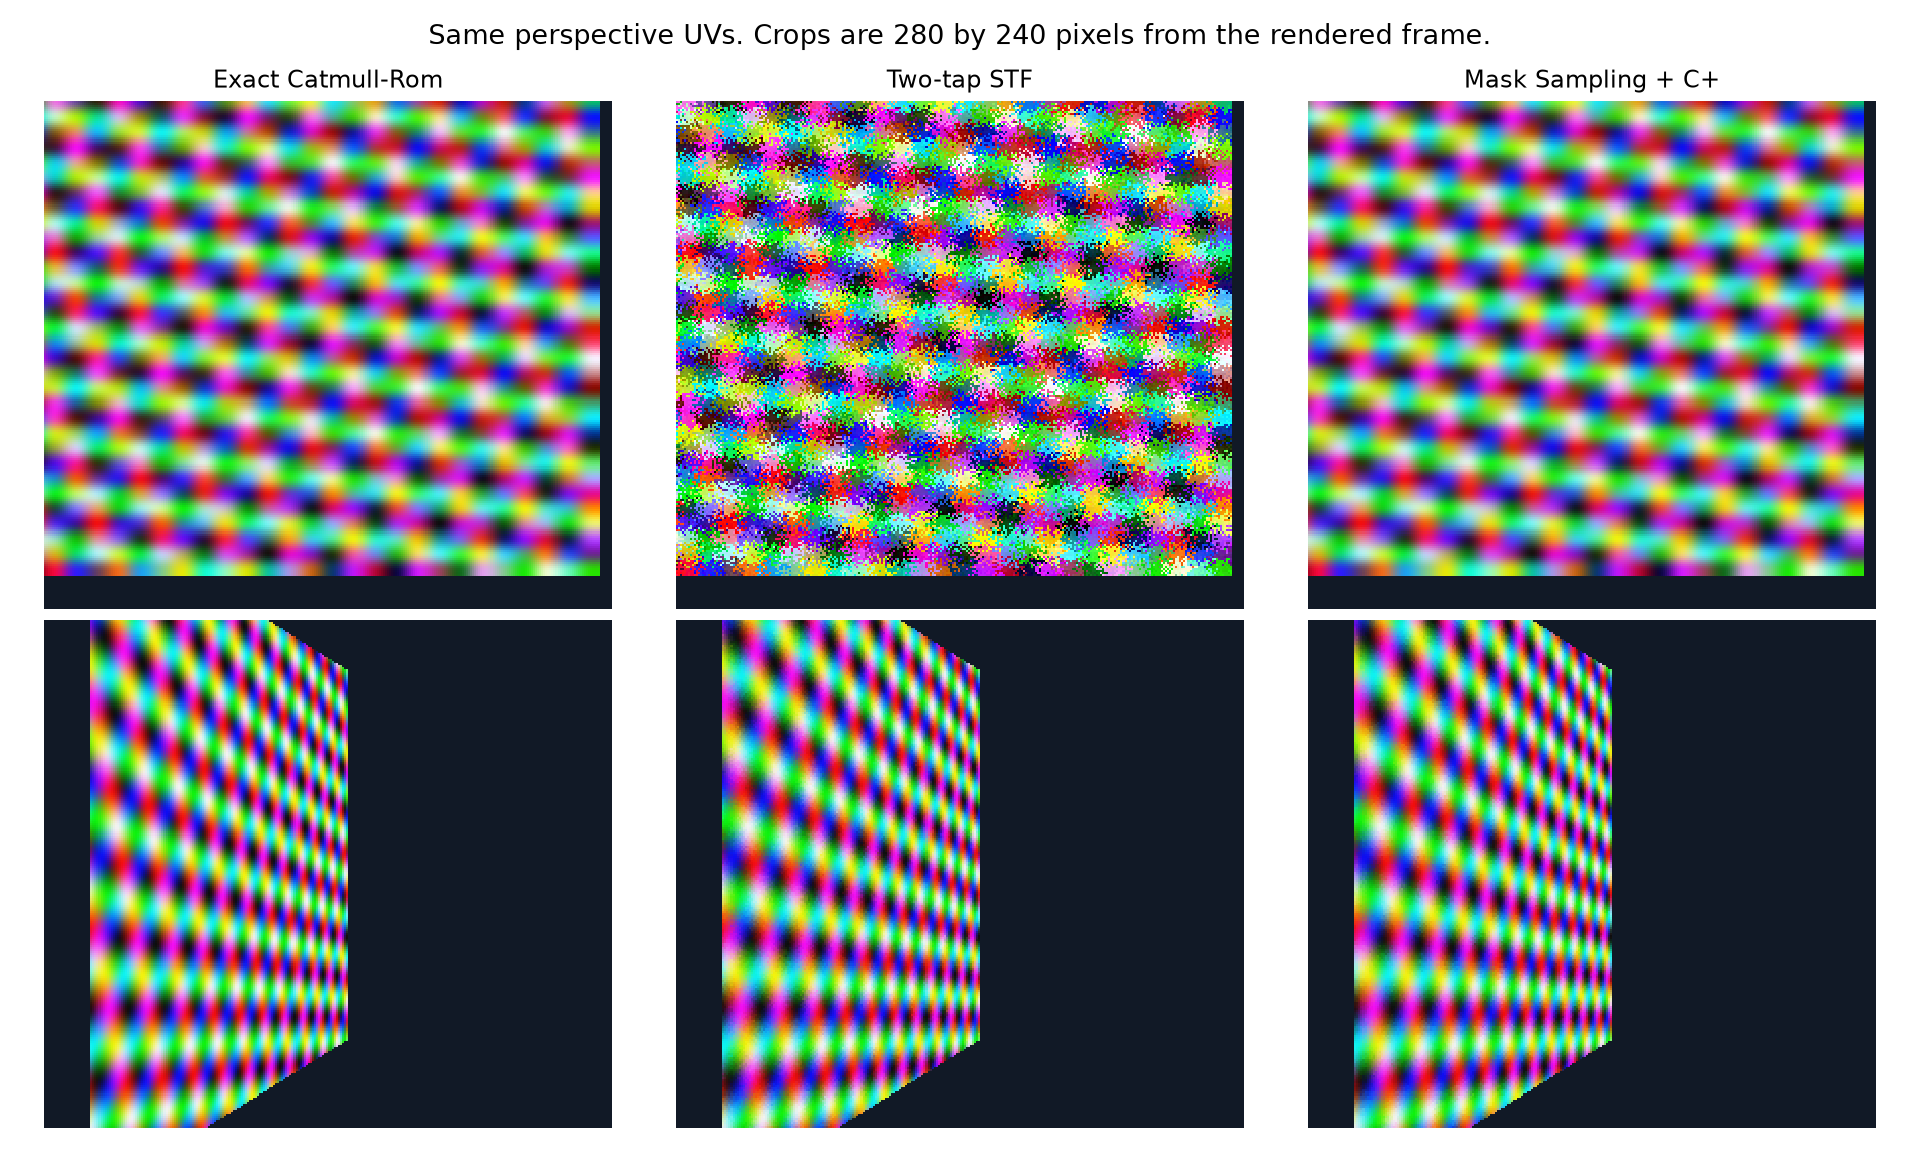
\includegraphics[width=\textwidth]{figures/comparison_sota.png}
\caption{The same $280\times240$ crop. Top: $32\times32$ texture at $0^\circ$, where Mask Sampling reproduces Catmull--Rom and two-tap STF is noisy. Bottom: $512\times512$ texture at $70^\circ$, where the tile budget cannot hold the footprint and the three reconstructions converge.}
\label{fig:sota}
\end{figure}

A separate check confirms the decision rule. On a synthetic tile whose 32 pixels share one footprint, the collaborative result matches the 16-tap filter to the last bit and uses at most 32 evaluations. A constant texture is reproduced to $10^{-16}$. The mean of 4000 two-tap draws on one probe lies within $0.006$ of the cubic color in every channel.

\section{Discussion}
The first experiment confirms the role of perspective correction. When clip-space $w$ varies across the surface, screen-space linear interpolation does not preserve the relationship between texture coordinates and the 3D surface. The reciprocal-$w$ correction compensates for this variation. The second experiment separates that geometric choice from the reconstruction budget. Under magnification, sharing the Catmull--Rom footprint inside an $8\times4$ tile reproduces the 16-tap filter with well under one evaluation per pixel. Under minification the same budget is too small for a $4\times4$ support, C+ remains only a modest improvement on two-tap sampling, and neither one is an antialiasing filter.

The project uses one planar quad and synthetic textures. The collaborative path is a CPU tile model with logical evaluation counts, so those counts are not GPU timings, cache misses, or bandwidth. Lighting, mipmaps, near-plane clipping, imported models, wave intrinsics, neural texel decoding, and denoising are outside this implementation. The analytic comparison evaluates the continuous signal at a point. It does not integrate the signal over a pixel footprint, so the point reference is not area antialiasing.

The rasterizer provides a controlled comparison of affine and perspective-correct texture mapping. The two UV rules nearly agree when the plane faces the camera, and affine interpolation develops substantial UV error as the plane becomes oblique. With the perspective-correct UV held fixed, Mask Sampling plus the C+ fallback reproduces Catmull--Rom on full tiles whenever the shared footprint fits in one evaluation per pixel, and it loses that exactness once the texture is minified. Perspective-correct coordinates and a budgeted reconstruction therefore answer different parts of the texture-mapping problem.

\begin{thebibliography}{9}
\bibitem{course3} Computer Graphics course lecture 03, Rasterization, 2026.
\bibitem{course4} Computer Graphics course lecture 04, Spatial Transformations, 2026.
\bibitem{course5} Computer Graphics course lecture 05, Rotation, Perspective and Projection, 2026.
\bibitem{course6} Computer Graphics course lecture 06, Texture Mapping, 2026.
\bibitem{glsl} Khronos Group, \emph{The OpenGL Shading Language, Version 4.60.8}, section 4.3.9.\\
\url{https://registry.khronos.org/OpenGL/specs/gl/GLSLangSpec.4.60.html}
\bibitem{vulkan} Khronos Group, \emph{Vulkan Specification}, Polygon Rasterization, Triangle Data Interpolation.\\
\url{https://docs.vulkan.org/spec/latest/chapters/primsrast.html}
\bibitem{ctf} T. Akenine-M\"oller, P. Ebelin, M. Pharr, and B. Wronski, Collaborative Texture Filtering, High-Performance Graphics, 2025.\\
\url{https://arxiv.org/abs/2506.17770}
\bibitem{stf} M. Pharr, B. Wronski, M. Salvi, and M. Fajardo, Filtering After Shading With Stochastic Texture Filtering, \emph{Proc. ACM Comput. Graph. Interact. Tech.}, 2024.
\end{thebibliography}
\end{document}
